\subsection{Dalil Ptolemy}
    Diketahui sebuah segiempat siklis $ABCD$ maka berlaku
    $$AB \cdot CD + BC \cdot DA = AC \cdot BD.$$

\begin{center}
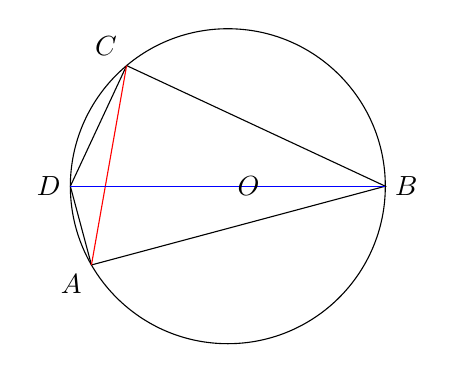
\begin{tikzpicture}
\coordinate (O) at (0,0);
\coordinate (B) at (0:2cm);
\coordinate (A) at (210:2cm);
\coordinate (D) at (180:2cm);
\coordinate (C) at (130:2cm);

\draw (O) circle (2cm);

\draw (A) -- (B) -- (C) -- (D) -- cycle;
\draw[red] (A) -- (C);
\draw[blue] (B) -- (D);

\node[right] at (B) {$B$};
\node[below left] at (A) {$A$};
\node[left] at (D) {$D$};
\node[above left] at (C) {$C$};
\node[right] at (O) {$O$};
\end{tikzpicture}
\end{center}

\subsection{Latihan Soal Dalil Ptolemy}
\begin{enumerate}
    \item Diberikan sebuah segiempat siklis $ABCD$ dengan $ABC$ adalah segitiga sama sisi. Jika $AD=2$ dan $CD=3$, panjang $BD=\dots$
\end{enumerate}